\documentclass[dvipdfmx,titlepage,a4j]{jsarticle}

\usepackage[top=20mm,bottom=20mm,left=20mm,right=20mm]{geometry}


\usepackage{url}
\usepackage{graphicx}
\usepackage{listings,jvlisting}
\usepackage{amsmath,amssymb}
\usepackage{graphicx}
\usepackage[yen]{okuverb}
\usepackage{ascmac}
\usepackage{fancybox}
\usepackage{fancyvrb}
\usepackage{fancyhdr}
\usepackage{lastpage}
\usepackage{caption}
\usepackage{subcaption}
\usepackage{here}
\usepackage{titling}

% ヘッダーとフッターの設定
\renewcommand{\headrulewidth}{0.2pt} % ヘッダーの線
\renewcommand{\footrulewidth}{0.4pt} % フッターの線

% ヘッダー
\fancyhead[L]{}
\fancyhead[C]{\thetitle}
\fancyhead[R]{}

% フッター
\fancyfoot[L]{}
\fancyfoot[C]{\thepage / \pageref{LastPage}} % ページ番号
\fancyfoot[R]{}

% lstlistingの設定
\lstset{
  language={C++},
  basicstyle={\ttfamily},
  identifierstyle={\small},
  commentstyle={\smallitshape},
  keywordstyle={\small\bfseries},
  ndkeywordstyle={\small},
  stringstyle={\small\ttfamily},
  frame={tb},
  tabsize={2},
  breaklines=true,
  columns=[l]{fullflexible},
  numbers=left,
  xrightmargin=0zw,
  xleftmargin=3zw,
  numberstyle={\scriptsize},
  stepnumber=1,
  numbersep=1zw,
  lineskip=-0.5ex
}

\title{超小型衛星向け光学ミッション設計の教科書}
\author{waarrk}
\date{2023年2月1日}

\begin{document}

\begin{titlepage}
    \centering
    \vspace*{2cm}

    \vspace{5cm}

    {\LARGE \textbf{小惑星表面探査を想定した\\CubeSat放出機構を使用して運用可能な自律移動型ローバー}}

    \vspace{0.5cm}

    {\textbf{千葉工業大学 先進工学部 未来ロボティクス学科}\\}
    {\textbf{22C1704 鷲尾 優作}}

    \vfill

    {\large 2025年5月7日}

    \vspace{1cm}
\end{titlepage}

\newpage

\section{本書の目的}
本計画書は、修士課程の研究計画を明確化し、指導教員との合意形成を図ることを目的とする。

\section{研究背景}
小惑星探査は近年、地球衝突天体への対処(プラネタリーディフェンス)や資源探査の観点から注目されている。
前者は小惑星や彗星の早期発見と特性評価を通じてリスクを排除することを目的とし、後者は希少鉱物や有用物質の採掘を通じて宇宙開発の基盤を形成する試みである。

一般的な小惑星探査機は、サンプル採取を目的としたミッション以外では、自機へのリスクを回避するため、小惑星表面への極端な接近を行わない。
そのため、多くのミッションにおいては上空からのリモートセンシングが主な観測手法となっている。このリモートセンシングは、光学カメラ、レーザー測距器、赤外線センサなどの機器を用いて行われるが、
小惑星表面の詳細な微細構造を完全に把握することには限界がある。
一方、日本の「はやぶさ2」では、表面にローバーを投下し、直接的なデータ収集が行われた。これにより表面画像の撮影に成功したが、
こうしたローバーの運用例は「MASCOT」や「MINERVA」に限られ、打上げ機会も稀であったため、運用数は数件しかなく、専用設計のため流用や転用も行われていない。

\begin{figure}[H]
    \centering
    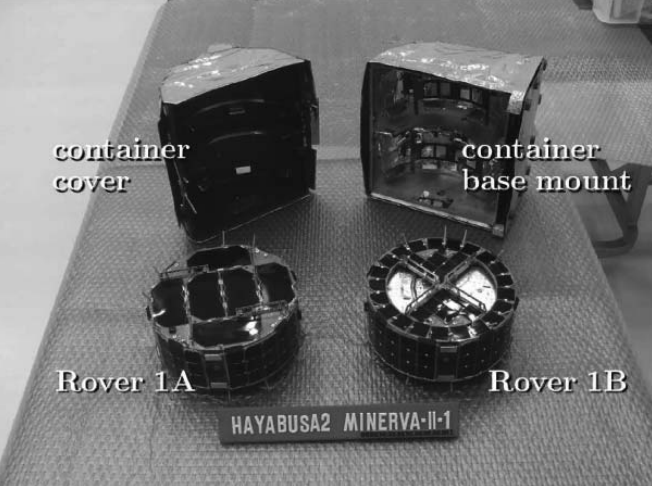
\includegraphics[width=0.3\textwidth]{picture/mine.png}
    \caption{小惑星探査機「はやぶさ2」に搭載されたローバー「MINERVA-II-1」}
    \label{fig:hayabusa2}
\end{figure}

近年、民間企業による宇宙探査技術の転用が進み、CubeSatのような小型衛星を活用した新たな探査手法が注目されている。
CubeSatは1U(10cm立方)を基本単位とした衛星であり、観測や通信など様々な用途に応用されている。
たとえば欧州宇宙機関の「Hera」探査機には2機のCubeSatが搭載され、また2028年にはExLabs社の「SERV」ミッションに千葉工業大学製のCubeSat探査機が搭載予定である。
ただし後者の探査機には自律移動能力がない。

将来的には、小型かつ自律移動可能な複数の探査機を展開し、広域から効率的なデータ収集を行うことが求められる。
本研究では、その実現を目指し、CubeSat放出機構を使用して運用可能な自律移動型ローバーの開発を目的とする。


\section{研究目的}
CubeSat放出機構を使用して運用可能な自律移動型ローバーを設計・開発し、小惑星表面における実用的な移動技術の確立を目指す。

\section{研究内容}
本研究では、CubeSatの放出機構に適合するロボットの開発を行う。
現在進行中のアポフィス向け探査機の設計成果を基に、同天体の物理特性を想定した設計を進める。スケジュールは表\ref{tab:schedule}に示す。

\begin{table}[H]
    \centering
    \caption{スケジュール案}
    \begin{tabular}{c|c|c|c}
        \hline
        期間           & 内容                     & 進捗   & 備考          \\
        \hline \hline
        2025年4月から12月 & 文献調査・アポフィス向け小惑星表面探査機開発 & 10\% & 先行研究の調査     \\
        \hline
        2026年1月から3月  & 具体的な後継機の仕様検討           & 0\%  & 機体設計、機構設計   \\
        \hline
        2026年4月頃から   & 試作機構造設計                & 0\%  & 試作機の製作、試験   \\
        \hline
        2027年4月頃から   & 試作機ソフトウェア設計            & 0\%  & 実験、評価、改良    \\
        \hline
        2027年10月頃    & 最終報告書作成                & 0\%  & 報告書の作成、発表準備 \\
        \hline
    \end{tabular}
    \label{tab:schedule}
\end{table}

要求される主な仕様を表\ref{tab:spec}に示す。


\begin{table}[H]
    \centering
    \caption{要求仕様}
    \begin{tabular}{c|c|c}
        \hline
        要求仕様   & 内容                       & 備考                  \\
        \hline \hline
        サイズ    & W6U(10cm x 20cm x 30cm)  & CubeSat規格準拠         \\
        \hline
        重量     & 12kg以下                   & CubeSat規格準拠         \\
        \hline
        自律移動機能 & GPS、IMU、LiDAR等を用いた自律移動機能 & 自律的な移動を実現するために必要な機能 \\
        \hline
    \end{tabular}
    \label{tab:spec}
\end{table}

\section{研究方針}
2025年度に行うアポフィス探査を想定した設計が完了し次第、後継機として仕様の検討、開発を行う。
本研究では、アポフィスの物理特性を考慮し、特に重力が小さい環境下での移動機構を重視する。
したがって、表面低重力下での安定移動を実現するための機構選定が重要となる。

\section{課題・リスク}
設計・開発に伴う主な課題とリスクを表\ref{tab:issue}に示す。

\begin{table}[H]
    \centering
    \caption{課題とリスク}
    \begin{tabular}{c|c}
        \hline
        項目     & 内容                   \\
        \hline \hline
        サイズ・重量 & 規格に準拠した制約内での設計が必要    \\
        駆動系設計  & 宇宙用駆動機構の開発経験不足       \\
        自律機能   & 小惑星特有の環境下でのナビゲーション技術 \\
        \hline
    \end{tabular}
    \label{tab:issue}
\end{table}

\section{期待される成果}
本研究の成果として、実運用に転用可能な探査機のプロトタイプが得られる見込みである。
CubeSatベースの汎用設計とすることで、実ミッションへの迅速な適用が期待される。

\newpage

\nocite{*}
\bibliographystyle{jplain}
\bibliography{refs}

\end{document}
